\documentclass[border=5pt]{standalone}
\usepackage[T1]{fontenc}
\usepackage[utf8]{inputenc}
\usepackage{amsmath}
\usepackage{graphicx}
\usepackage{tikz}
\usetikzlibrary{positioning,arrows.meta,calc,shapes.geometric}

\begin{document}
\resizebox{!}{90mm}{%
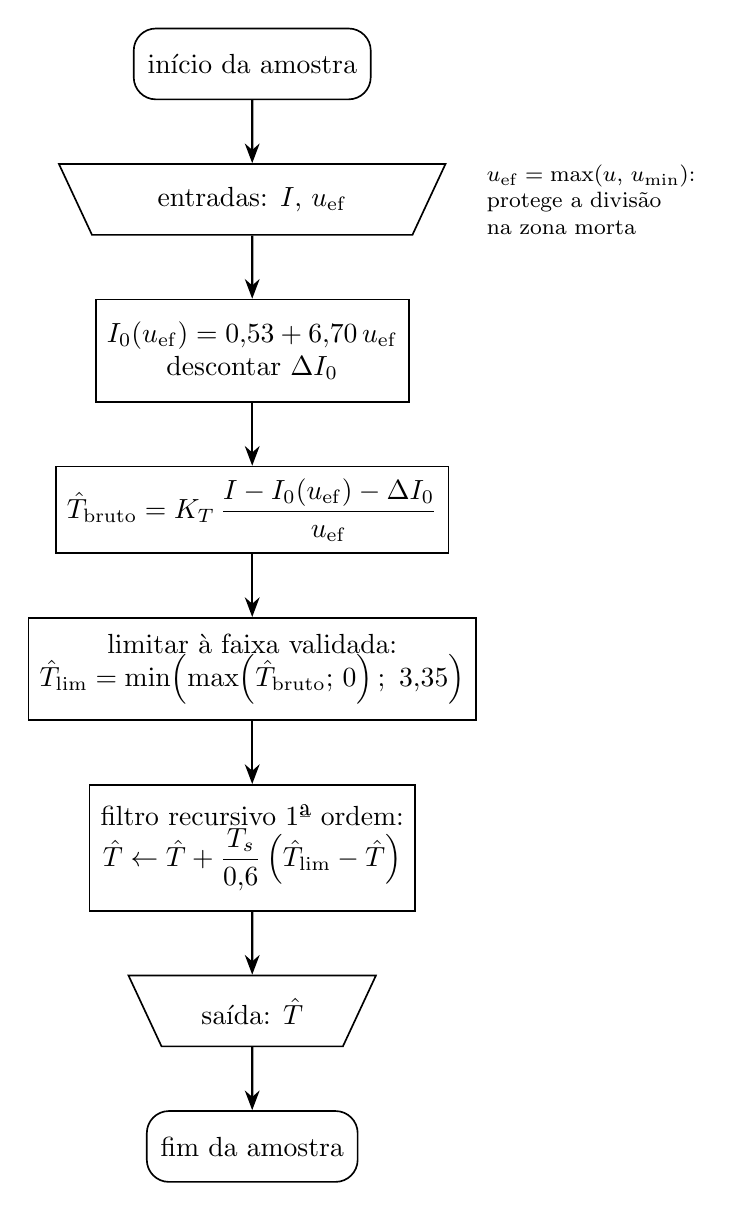
\begin{tikzpicture}[
  font=\normalsize,
  term/.style={draw=black, semithick, rounded corners=8pt, minimum height=9mm, inner sep=5pt, align=center},
  block/.style={draw=black, semithick, minimum height=11mm, minimum width=30mm, inner sep=4pt, align=center},
  io/.style={draw=black, semithick, trapezium, trapezium angle=65, shape border rotate=180, minimum height=9mm, inner sep=4pt, align=center},
  decision/.style={diamond, draw=black, semithick, aspect=2.6, inner sep=1pt, align=center},
  lab/.style={font=\footnotesize\itshape},
  arr/.style={-{Stealth[length=2.5mm]}, thick},
  node distance=8mm]
\node[term] (ini) {início da amostra};
\node[io, below=of ini] (ent) {entradas: $I$, $u_{\mathrm{ef}}$};
\node[font=\footnotesize, right=6mm of ent, align=left] (entnota) {$u_{\mathrm{ef}} = \max(u,\,u_{\min})$:\\protege a divisão\\na zona morta};
\node[block, below=of ent, minimum height=13mm] (i0) {$I_0(u_{\mathrm{ef}}) = 0{,}53 + 6{,}70\,u_{\mathrm{ef}}$\\descontar $\Delta I_0$};
\node[block, below=of i0] (bruto) {$\hat{T}_{\mathrm{bruto}} = K_T\,\dfrac{I - I_0(u_{\mathrm{ef}}) - \Delta I_0}{u_{\mathrm{ef}}}$};
\node[block, below=of bruto, minimum height=13mm] (lim) {limitar à faixa validada:\\$\hat{T}_{\mathrm{lim}} = \min\!\left(\max\!\left(\hat{T}_{\mathrm{bruto}};\,0\right);\ 3{,}35\right)$};
\node[block, below=of lim, minimum height=16mm] (filtro) {filtro recursivo 1ª ordem:\\$\hat{T} \leftarrow \hat{T} + \dfrac{T_s}{0{,}6}\left(\hat{T}_{\mathrm{lim}} - \hat{T}\right)$};
\node[io, below=of filtro] (saida) {saída: $\hat{T}$};
\node[term, below=of saida] (fim) {fim da amostra};
\draw[arr] (ini) -- (ent);
\draw[arr] (ent) -- (i0);
\draw[arr] (i0) -- (bruto);
\draw[arr] (bruto) -- (lim);
\draw[arr] (lim) -- (filtro);
\draw[arr] (filtro) -- (saida);
\draw[arr] (saida) -- (fim);
\end{tikzpicture}}
\end{document}
